\chapter{Marco Teórico-Conceptual}\label{chapter:state-of-the-art}
Un negocio maneja grandes volúmenes de información de todo tipo,  la gestión de la misma es un factor esencial para su éxito. De ahí la importancia de contar con sistemas de información que permitan el control, visibilidad, orden, disposición y vinculación de todo ese movimiento de datos. A partir de estas necesidades surgen una serie de conceptos, modelos y tecnologías, cuyo estudio es necesario para poder explotar al máximo las facilidades que ofrecen. En el presente capítulo se discuten brevemente aquellos que constituyen el fundamento teórico y metodológico para el desarrollo de esta investigación.

\section*{Gestión del Conocimiento}\label{gestion_conocimiento}
\addcontentsline{toc}{section}{Gestión del Conocimiento}
Con el auge del internet las tecnologías experimentan cambios monumentales para ayudar a las organizaciones a optimizar sus procesos y realizar transacciones  comerciales de manera más eficiente. Ejemplo de ello ha sido en la tecnología de la información ya que los volúmenes de datos se encuentran en crecimiento exponencial y con estos se han desarrollado cada vez más interrogantes de como almacenarlos de manera eficiente para aprovechar e incrementar su valor.\\

La gestión del conocimiento (GC) está encargada de organizar y gestionar la información de manera eficaz, esta tiene el fin de transferir el conocimiento desde el lugar donde es generado hasta donde será asimilado, valorado, transferido y posteriormente utilizado tratando de mantener la eficiencia para maximizar y aprovechar su valor. Este es un proceso que asegura la aplicación y desarrollo de conocimientos pertinentes de una empresa para contribuir a la sostenibilidad competitiva de la misma, la solución de problemas y mantener su capacidad (Andreu \& Sieber 1999). Para desarrollarla es necesario que en la empresa madure la cultura empresarial y organizacional, se disponga de equipos humanos convenientemente preparados y se utilice una metodología de desarrollo que facilite el análisis, diseño, instrumentación, puesta en producción y control de proyectos con la disposición de herramientas informáticas. Sin estas condiciones, no es posible garantizar una acertada gestión del conocimiento.\\

Aproximadamente el 81\% de las empresas más grandes de los Estados Unidos utilizan diversas formas de GC (Becerra-Fernández \& Sabherwal, 2001), sin embargo se plantea que muchas organizaciones ha sido difícil implementarlas y mantener programas eficaces dado que la estimación de fallo oscila entre el 50\% y 70\% (Turban et al., 2005). De igual forma se indica que existen algunas experiencias positivas con respecto a este sistema ya que es practicado en el 80\% de las organizaciones alrededor del mundo. La GC no es tarea fácil para las organizaciones fácil debido a la complejidad de identificar, valorar e implementar el conocimiento pertinente para obtener ventajas competitivas, pero tampoco es una meta imposible (De Freitas \& Yaber, 2015). Una de las aplicaciones más extendidas tiene lugar en los sistemas de toma de decisiones, que generalmente se enfocan en estrategias de inteligencia empresarial. La inteligencia empresarial se ha convertido en un modelo de control y de crecimiento corporativo para lograr la sostenibilidad competitiva por su adaptabilidad a los cambios del mercado y la resolución de problemas a los clientes.

\section*{Inteligencia de Negocios}\label{BI}
\addcontentsline{toc}{section}{Inteligencia de Negocios}
hola

\section*{Modelos de datos}\label{models}
\addcontentsline{toc}{section}{Modelos de datos}
Una solución de inteligencia de negocios se alimenta de los datos transaccionales que se generan en la empresa en su accionar diario, además de datos obtenidos en fuentes externas de las que puede disponer. Los sistemas transaccionales de una organización recogen de manera sistemática grandes volúmenes de datos que describen los principales procesos del negocio, con lo cual se satisfacen las necesidades operacionales de la empresa. (Bernabeu, 2010)\\

Los datos almacenados en los sistemas transaccionales son transformados en información, dada la diversidad y la heterogeneidad de las fuentes de datos y los formatos, esta información es demasiado compleja y difícil de extraer de manera que sea efectiva. Luego, es preciso organizar, consolidar y almacenar los datos para después transformarlos y extraer conocimiento y para esto se debe determinar el modelo de datos adecuado para su almacén y futuras consultas para la extracción de este mismo conocimiento.

\section*{Modelo Multidimencional}\label{multidim_model}
\addcontentsline{toc}{section}{Modelo Multidimencional}
Un modelo de datos diseñado para el desarrollo de una BI debe sintetizar la lógica del negocio con vistas a brindar a los analistas información centralizada y resumida como apoyo a la toma de decisiones, mostrándose esta de la forma más rápida y fiable. El modelo relacional para la normalización de los datos atenta contra la simplicidad y eficiencia del proceso analítico en los sistemas transaccionales, por tanto se evidencia el surgimiento de modelos dimensionales para la trata de los datos. Contrario a lo que muchos afirman, el enfoque dimensional no fue creado por Ralph Kimball, los términos asociados a este modelo fueron producidos en los 60’s en un proyecto de investigación conjunto entre la Universidad de Dartmouth y la empresa de productos alimenticios General Mills. (Kimball, et al., 2002 p. 16)\\

Conceptualmente, este modelo define una estructura multidimensional de la información semejante a los sujetos de análisis del negocio, empleando dos componentes fundamentales: los hechos y las dimensiones. Un hecho (del inglés, fact) es un dato numérico que describe el comportamiento del negocio. Los hechos se almacenan en tablas de hechos (del inglés, fact table). Una dimensión (del inglés, dimension) es un criterio de análisis que caracteriza el negocio y permite navegar por la información localizada en las tablas de hechos. Cada dimensión es representada por una tabla en el modelo, conocida como tabla de dimensión (del inglés, dimension table). (Kimball, et al., 2002) \\

Una tabla de hechos está compuesta por medidas numéricas relacionadas con un conjunto de tablas de dimensiones. Es por ello que una tabla de hechos posee una llave primaria compuesta por llaves foráneas a las dimensiones que intervienen en el sujeto del negocio que se está modelando, expresando una relación muchos a muchos entre las dimensiones. (Kimball, et al., 2002). Estas también son vistas como las encargadas de almacenar observaciones o eventos, y pueden ser, por ejemplo, pedidos de ventas, existencias, tasas de cambio, temperaturas, etc. Una tabla de hechos contiene columnas de clave de dimensiones relacionadas con las tablas de dimensiones y columnas de medida numéricas. Las columnas de clave de dimensiones determinan la dimensionalidad de una tabla de hechos, mientras que los valores de clave de dimensiones determinan la granularidad de una tabla de hechos.\\

Las tablas de dimensiones describen entidades empresariales (las cosas que se modelan). Las entidades pueden incluir productos, personas, lugares y conceptos, incluido el propio tiempo. La tabla más coherente de un esquema de estrella es una tabla de dimensiones de fecha. Una tabla de dimensiones contiene una columna (o columnas) de clave que actúa como identificador único y columnas descriptivas.\\

Una estructura multidimensional puede ser modelada a través de dos esquemas principales:

\begin{itemize}
\item \textbf{Esquema de Estrella:} el centro de la estrella es la tabla de hechos y las puntas son las tablas de dimensiones del cubo, un ejemplo de su visualización seria el visto en la Figura 1.1
\item \textbf{Esquema de Copo de Nieve:} es una variación del esquema de estrella en la cual se normalizan algunas de las dimensiones esencialmente con el objetivo de representar las jerarquías involucradas de manera explícita, Figura 1.2
\end{itemize}


\begin{figure}[ht]
  \begin{center}
    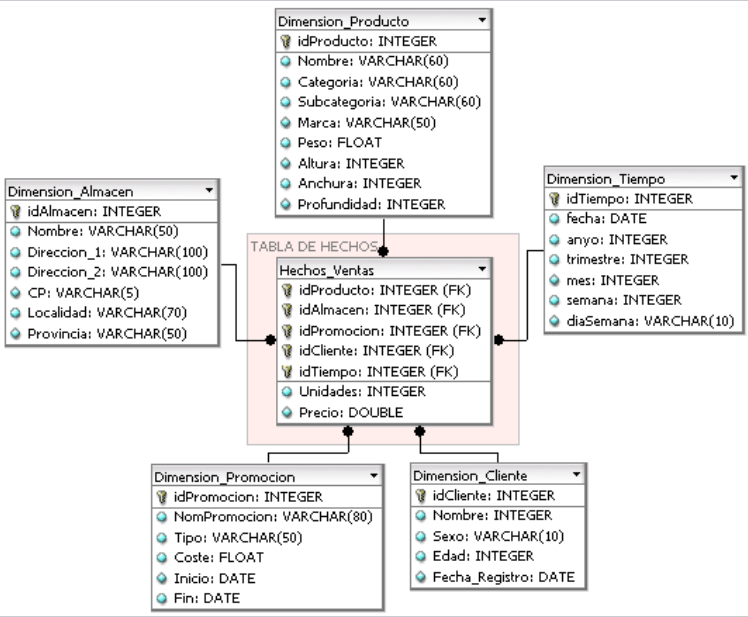
\includegraphics[scale=0.35]{Graphics/figura1_1.png}
    \caption{Ejemplo visual de un Esquema de Estrella (Imagen obtenida de la Wikipedia)}
    \label{fig:estrella}
  \end{center}
\end{figure}

\begin{figure}[ht]
  \begin{center}
    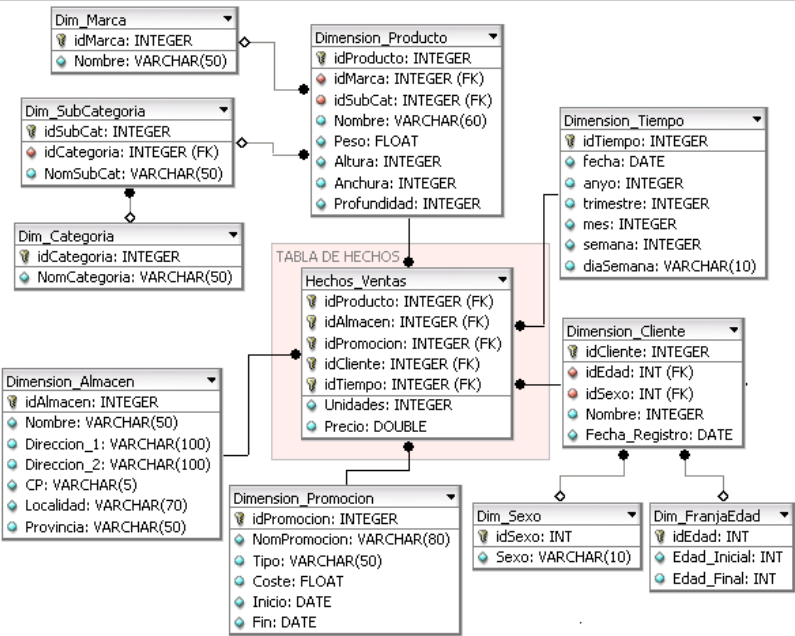
\includegraphics[scale=0.35]{Graphics/figura1_2.png}
    \caption{Ejemplo visual de un Esquema de Copo de Nieve (Imagen obtenida de la Wikipedia)}
    \label{fig:estrella}
  \end{center}
\end{figure}

Otra de las ventajas del modelo dimensional es la posibilidad de filtrar los datos de modo sencillo, extrayendo un subconjunto del conjunto de los datos para análisis más detallados (slicing and dicing)\\


\begin{figure}[ht]
  \begin{center}
    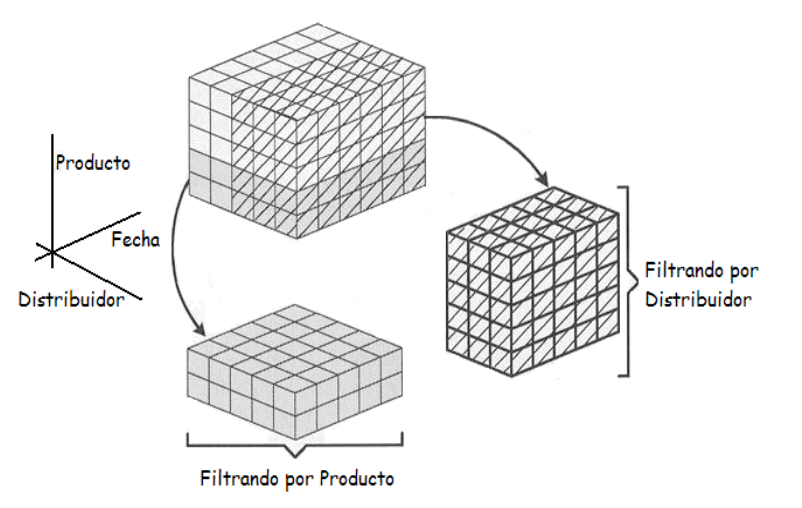
\includegraphics[scale=0.4]{Graphics/figura1_3.png}
    \caption{Reduciendo el espacio de análisis. (Giovinazzo, 2000)}
    \label{fig:cubo}
  \end{center}
\end{figure}

%%
% IMAGEN
%%


El enfoque multidimensional incluye además los siguientes conceptos:
\begin{itemize}
\item \textbf{Medidas:} Las medidas o métricas son los hechos y las sumarizaciones preestablecidas que se efectúan sobre los hechos y que se crean utilizando funciones de agregación, funciones matemáticas, funciones estadísticas, operadores matemáticos y lógicos. Las medidas pueden ser aditivas, semiaditivas o no aditivas: (Kimball, et al., 2002)
\item \textbf{Atributos:} Los atributos expresan las propiedades y/o las características de las dimensiones. 
\item \textbf{Jerarquías:} Una jerarquía representa un orden parcial que se establece en una dimensión y que se expresa mediante una estructura arbórea. La principal ventaja de establecer relaciones jerárquicas en una dimensión reside en la navegación por los datos al desplazarse en profundidad por el árbol correspondiente.
\end{itemize}

El rendimiento de un sistema de gestión de bases de datos (DBMS, Database Management System) está directamente relacionado con la eficiencia del almacenamiento de datos en disco y su movimiento hacia los registros de CPU para el procesamiento. El modelo dimensional fue instrumentado exitosamente en la época de los servidores de 32 bits, con uno o dos procesadores y menos de un gigabyte de RAM, cuando el almacenamiento por filas era la única opción para las bases de datos (Russo et al., 2012). \\

En búsqueda de la eficiencia de estos procesos, ha crecido el interés en el almacenamiento orientado a columnas (column-oriented storage). En este tipo de distribución cada página de datos contiene los valores correspondientes a una sola columna y, al tratarse de datos estructurados, en el proceso de indización se conservan los valores repetidos solo una vez, todo lo cual favorece la compresión y rápida recuperación. Las comparaciones entre las bases de datos orientadas a filas y a columnas suelen estar relacionadas con la eficiencia del acceso al disco duro para una carga de trabajo determinada, ya que el tiempo de búsqueda es increíblemente largo en comparación con otros cuellos de botella en las computadoras.


\section*{Python y Django}\label{py_dj}
\addcontentsline{toc}{section}{Python y Django}
Junto con los avances computacionales y el auge de las tecnologías orientadas al código abierto la corporación CIMEX ha tomado como decición ser parte de las empresas que se suman a este ámbito.



